% ============================================================
%  Chapter 3: Design and Implementation
% ============================================================

\chapter{Design and Implementation}
\label{chap:implementation}

% ============================================================
%  Section 3.1 — Overview of the pipeline
% ============================================================
\section{Overview}
\label{sec:overview}

The reproduction is implemented as a Python package, \texttt{ct\_tfpnp}, that integrates with the LION toolbox~\citep{Biguri2024LION} for the CT geometry, forward operator, and dataset handling. The package contains
all the components of the TFPnP algorithm, including the ResNet-18 policy network, the residual value network, the ADMM environment, the DRUNet denoiser wrapper, and the RL training loop, as well as the baseline reconstruction methods (FBP, TV, DRUNet alone, FBPConvNet, and Fixed PnP-ADMM) used for comparison.

The full experimental pipeline covers eleven trained TFPnP runs and two baseline model checkpoints (FBPConvNet and a CT-trained DRUNet), with each run producing a set of diagnostic figures via \texttt{scripts/evaluate\_run.py}, including training curves, per-image metrics, policy behaviour, and a reconstruction gallery. All experiments are launched on the Cambridge Service for Data Driven
Discovery (CSD3) HPC cluster through SLURM job scripts (see~\Cref{app:supplementary}), with outputs written to a results directory for analysis.

% ============================================================
%  Section 3.2 — Geometry, data, and noise conventions
% ============================================================
\section{Geometry, data, and noise conventions}
\label{sec:geometry-noise}

All experiments use a sparse 30-view parallel-beam geometry, matching~\citet{Wei2022TFPnP}. As LION had no matching preset, a custom \texttt{Geometry} object was constructed with 30 angles uniformly spaced over $[0, \pi)$, a $512 \times 512$ image, and 724 detectors ($[512\sqrt{2}]$, chosen to cover the image diagonal). The forward operator is LION's \texttt{CTProjectionOp}, a thin wrapper around tomosipo~\citep{Hendriksen2021Tomosipo}, whereas \citet{Wei2022TFPnP} use TorchRadon~\citep{Ronchetti2020TorchRadon}. The two are mathematically equivalent but differ in scaling conventions (\Cref{sec:admm-gradient}).

Training and evaluation data come from LIDC-IDRI~\citep{Armato2011LIDC}, split at the patient level into 80/10/10 partitions using LION's default loader. This yields approximately 3300, 401, and 389 slices in the training, validation, and test splits respectively, with up to 5 slices per patient and a 50/50 nodule-to-non-nodule ratio. \citet{Wei2022TFPnP} evaluate on 50 randomly selected lung slices from the COVID-19 CT lung and infection segmentation dataset~\citep{Ma2020COVID19}, making our test set substantially larger. \Cref{fig:sample_lidc} shows a representative training slice.

Image intensities are preserved in linear attenuation coefficient ($\mu$) units throughout the pipeline, with values approximately in $[0, 2.5]$\,cm$^{-1}$. This convention is set by LION's LIDC loader via its \texttt{from\_HU\_to\_mu} transform, and is preserved rather than rescaled to $[0, 1]$ as in many other reproductions, to retain the physical interpretation of reconstructed values.

Sinogram noise is added following~\citet{Wei2022TFPnP}'s percentage-of-signal-standard-deviation convention. For each ground truth image, the clean sinogram $y_{\text{clean}} = Ax_{\text{gt}}$ is normalised by a per-image factor $\text{SCALE} = y_{\text{clean}}.\text{max}() / x_{\text{gt}}.\text{max}()$ so that the percentage noise fraction applies consistently across images. Additive Gaussian noise is then applied at 5\%, 7.5\%, or 10\% of the normalised sinogram's standard deviation, and the result is rescaled back to the original operator range. Noise seeds are deterministic per image (\texttt{seed = img\_idx * 100}), so paired comparisons between methods use identical realisations.

LION provides a more physically realistic \texttt{sinogram\_add\_noise} routine based on a Poisson-Gaussian model, which would better represent the photon-counting statistics of real CT acquisitions, but it takes physical parameters (photon count, detector gain) rather than a percentage noise fraction, so its noise levels do not map directly onto the paper's 5\%, 7.5\%, 10\% conditions. The paper's percentage convention is used here to keep the implementation as close to~\citet{Wei2022TFPnP}'s as possible and preserve the direct comparability of results.

One consequence of retaining native $\mu$ units is that PSNR values in this report are approximately $5$\,dB higher than those reported in~\citet{Wei2022TFPnP}, affecting cross-study comparisons but not within-experiment rankings (\Cref{sec:metrics}).

% ------------------------------------------------------------
%  Figure 3.1: Sample training image (lung slice) from LIDC
% ------------------------------------------------------------
\begin{figure}[H]
    \centering
    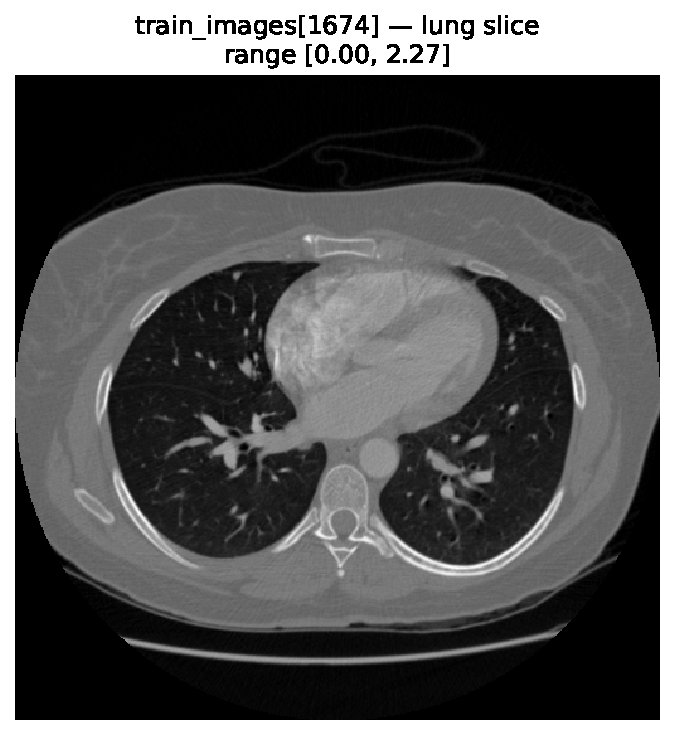
\includegraphics[width=0.5\linewidth]{../figures/12/01_sample_train_image.pdf}
    \caption{A lung slice from the LIDC-IDRI training split, in native $\mu$ units (approximately $[0,2.3]$\,cm$^{-1}$).}
    \label{fig:sample_lidc}
\end{figure}

% ============================================================
%  Section 3.3 — TFPnP policy and RL training
% ============================================================
\section{TFPnP policy and RL training}
\label{sec:tfpnp-policy}

The TFPnP policy network follows the architecture described by~\citet{Wei2022TFPnP}. A ResNet-18 backbone extracts features from a five-channel input consisting of the current ADMM iterates $(x, z, u)$, a noise-level map, and an iteration-progress map. Two output heads share the resulting 512-dimensional feature vector, a two-way termination head predicting whether to stop, and a parameter head predicting the next $m = 5$ pairs of $(\sigma, \mu)$ via a sigmoid activation rescaled to the configured action ranges.

The backbone follows torchvision's ResNet-18, with only the first convolutional layer replaced to accept five input channels rather than three. Table~1 of~\citet{Wei2022TFPnP} specifies a $3 \times 3$ stem, whereas torchvision's default is $7 \times 7$, which is retained for this implementation. Our slices are $512 \times 512$, so layer4 emits $16 \times 16$ rather than $4 \times 4$, but an adaptive average pool absorbs the difference. Both deviations are recorded in~\Cref{tab:implementation-differences}.

Table~1 gives conv1 an output of $64 \times 64$ and layer1 an output of $32 \times 32$, but does not state how this is obtained, since a standard ResNet-18's layer1 does not downsample. We retain torchvision's max-pooling layer, which reproduces the stated output sizes.

The value network departs from the paper. The caption of Table~1 specifies the same feature extractor as the policy, with batch normalisation replaced by weight normalisation and ReLU replaced by TReLU. Our value network is instead a residual network of eight blocks at constant width 64, with no normalisation, standard ReLU activations, no spatial downsampling, and a final linear layer mapping a 64-dimensional feature vector to the scalar value estimate. It preserves the paper's removal of batch normalisation but not the replacements specified alongside it. The consequences of this divergence are analysed in~\Cref{sec:in-domain-gap}.

Policy action ranges are $\sigma \in [1, 5]$ and $\mu \in [10, 100]$. The $\sigma$ range is calibrated to the natural-image DRUNet's useful operating region for CT, identified from a preliminary sensitivity sweep (\Cref{sec:calibration}) in which $\sigma > 5$ over-smoothed reconstructions. The $\mu$ range balances against the normalised data-fidelity gradient (\Cref{sec:admm-gradient}), with \citet{Wei2022TFPnP}'s corresponding effective range set at $[0.01, 1]$ because their unnormalised gradient is $\sim 100\times$ smaller.

The RL formulation matches~\citet{Wei2022TFPnP}'s equations 15--17. The value network is trained on a temporal-difference (TD) loss, which regresses each state's value estimate towards the reward received plus the discounted estimate of the next state, with discount factor $\gamma = 0.99$. Stability is maintained by comparing against a target network, a slowly-updated copy of the value network, refreshed by exponential moving average at rate $10^{-3}$. The termination policy $\pi_1$ uses a value baseline, subtracting the value network's prediction from the reward before applying the REINFORCE update, which reduces gradient variance. The reward is $r = \Delta\text{PSNR} - \eta$ with $\eta = 0.05$.

Learning rates are $10^{-4}$ for the critic, $3 \times 10^{-5}$ for the shared policy features and termination head, and $10^{-6}$ for the parameter head, the last kept low to compensate for the sensitivity of $\pi_2$'s gradient through the ADMM rollout. The paper's hyperparameters $m = 5$, $N = 6$, and $\eta = 0.05$ are preserved exactly.

% ============================================================
%  Section 3.4 — ADMM step and z-step gradient normalisation
% ============================================================
\section{ADMM step and z-step gradient normalisation}
\label{sec:admm-gradient}

The ADMM environment implements~\citet{Wei2022TFPnP}'s equations 7--9, with each outer iteration performing three sub-steps. The $x$-step applies the DRUNet denoiser as an implicit image prior, the $z$-step enforces data fidelity against the noisy sinogram, and the $u$-step updates the dual variable to accumulate constraint violation.

The $z$-step is solved by six iterations of gradient descent, so that the update is differentiable end-to-end. The model-based DDPG update for $\pi_2$ requires backpropagation through the entire $z$-step, which gradient descent supports through automatic differentiation.

LION's adjoint operator $A^{\top}$ implements the raw backprojection of tomosipo's discrete Radon transform, summing sinogram values along ray paths without normalisation, so $A^{\top}(Az)$ produces per-voxel values much larger than the input image. Without adjustment, the data-fidelity gradient $A^{\top}(Az - y)$ would dominate the proximal term $\mu(z - \text{target})$ for any reasonable $\mu$, rendering the policy's $\mu$ predictions meaningless. To resolve this, the backprojected residual is normalised to unit maximum before being combined with the proximal term,

\begin{equation}
\text{grad} = \frac{A^{\top}r}{\|A^{\top}r\|_\infty + \epsilon} +
              \mu(z - \text{target}),
\end{equation}

where $r = Az - y$ is the sinogram residual and $\epsilon = 10^{-8}$ prevents division by zero. The proximal term pulls $z$ towards the current ADMM estimate $\text{target} = x + u$, with $\mu$ controlling the strength. Normalising the first term places its magnitude on the same scale as the proximal term, so $\mu$ can meaningfully balance the two. The gradient step size is further scaled as $\alpha / (1 + \mu)$, with $\alpha = 1$, to keep the update bounded as $\mu$ grows. Our absolute $\mu$ values therefore differ from~\citet{Wei2022TFPnP}'s in scale but preserve their role in the ADMM balance, as reflected in the $\mu \in [10, 100]$ action range (\Cref{sec:tfpnp-policy}).

% ============================================================
%  Section 3.5 — Baselines
% ============================================================
\section{Baselines}
\label{sec:baselines}

The TFPnP reproduction is validated against five baseline methods. Three of the paper's baselines (RED-CNN, LPD, RPGD) are either absent from LION or would require training beyond the project timeline, so were not included.

\textbf{FBP} applies a Ram-Lak filter followed by unfiltered backprojection through LION's operator, with the analytical normalisation $\pi / (2N)$ for $N = 30$ projection angles. The result is clamped to non-negative values.

\textbf{TV reconstruction} uses ISTA with 200 iterations and anisotropic total variation at regularisation strength $\lambda = 0.01$. The data-fidelity gradient is normalised to unit maximum before each step, matching the ADMM z-step convention (\Cref{sec:admm-gradient}), and non-negativity is enforced after each iteration.

\textbf{DRUNet alone} applies the natural-image DRUNet as a single denoising pass over the FBP reconstruction, with fixed $\sigma = 10$. This is not one of~\citet{Wei2022TFPnP}'s baselines, but provides a useful lower bound, isolating how much of TFPnP's performance comes from ADMM's iterative refinement rather than the denoiser itself.

\textbf{FBPConvNet}~\citep{Jin2017FBPConvNet} is a five-stage U-Net mapping sparse-view FBP reconstructions to full-view ground truth. Our FBPConvNet is trained end-to-end on the LIDC training split (250 patients across 80 epochs) using LION's implementation, with MSE loss and Adam at learning rate $10^{-4}$, at a fixed 5\% sinogram noise level. This departs both from~\citet{Jin2017FBPConvNet}'s original protocol (clean projections at training, noise added at inference) and from~\citet{Wei2022TFPnP}'s FBPconv, whose near-constant PSNRs across noise levels (23.00, 22.94, 22.86\,dB) implies mixed-noise training, although this is not explicitly stated. Fixed 5\% training makes evaluation at 7.5\% and 10\% out-of-distribution, and is central to the reversal narrative in~\Cref{sec:headline}.

\textbf{Fixed PnP-ADMM} uses the same ADMM environment as TFPnP with hand-calibrated $\sigma = 1.5$ and $\mu = 20$, selected as the operating point maximising PSNR on a preliminary sweep. Any improvement of TFPnP over Fixed PnP-ADMM can be attributed to policy-based hyperparameter adaptation.

% ============================================================
%  Section 3.6 — CT-specific DRUNet training
% ============================================================
\section{CT-specific DRUNet training}
\label{sec:ct-drunet}

The headline TFPnP result (\texttt{run\_04}) uses the natural-image DRUNet as denoiser prior, matching~\citet{Wei2022TFPnP}. As an extension, a CT-specific DRUNet is trained to test whether an in-domain denoiser improves reconstruction quality. The same architecture and checkpoint format as the pretrained natural-image DRUNet~\citep{zhang2021plug} is used, making it a drop-in replacement.

Training uses the LIDC training split (3300 slices) for 50 epochs with Adam at learning rate $10^{-4}$, a cosine annealing schedule, and batch size 8. Each mini-batch samples a random noise level $\sigma \in [0, 50]$ per image, following~\citet{zhang2021plug}'s multi-level convention, and loss is computed using mean squared error in the per-image $[0, 1]$ normalised space to match the DRUNet's input convention. Validation PSNR at $\sigma \in \{5, 15, 25\}$ is monitored throughout training, with best-checkpoint selection based on PSNR at $\sigma = 15$. \Cref{fig:ct_drunet_training} shows the training progression.

An initial drop-in test using the CT-DRUNet in place of the natural-image DRUNet within \texttt{run\_04}'s TFPnP pipeline revealed a calibration mismatch, with PSNR collapsing to approximately $13$\,dB, below the FBP baseline. Diagnosis showed that the CT-DRUNet's optimal $\sigma$ sits at approximately $8$, indicating that
the regularisation scale at which the denoiser is most useful shifts with the training data distribution. When each denoiser is compared at its calibrated optimum, the CT-DRUNet outperforms the natural-image DRUNet at every noise level, with an advantage that grows with noise (\Cref{sec:in-domain}).

% ------------------------------------------------------------
%  Figure 3.3: CT-DRUNet training curves
% ------------------------------------------------------------
\begin{figure}[H]
    \centering
    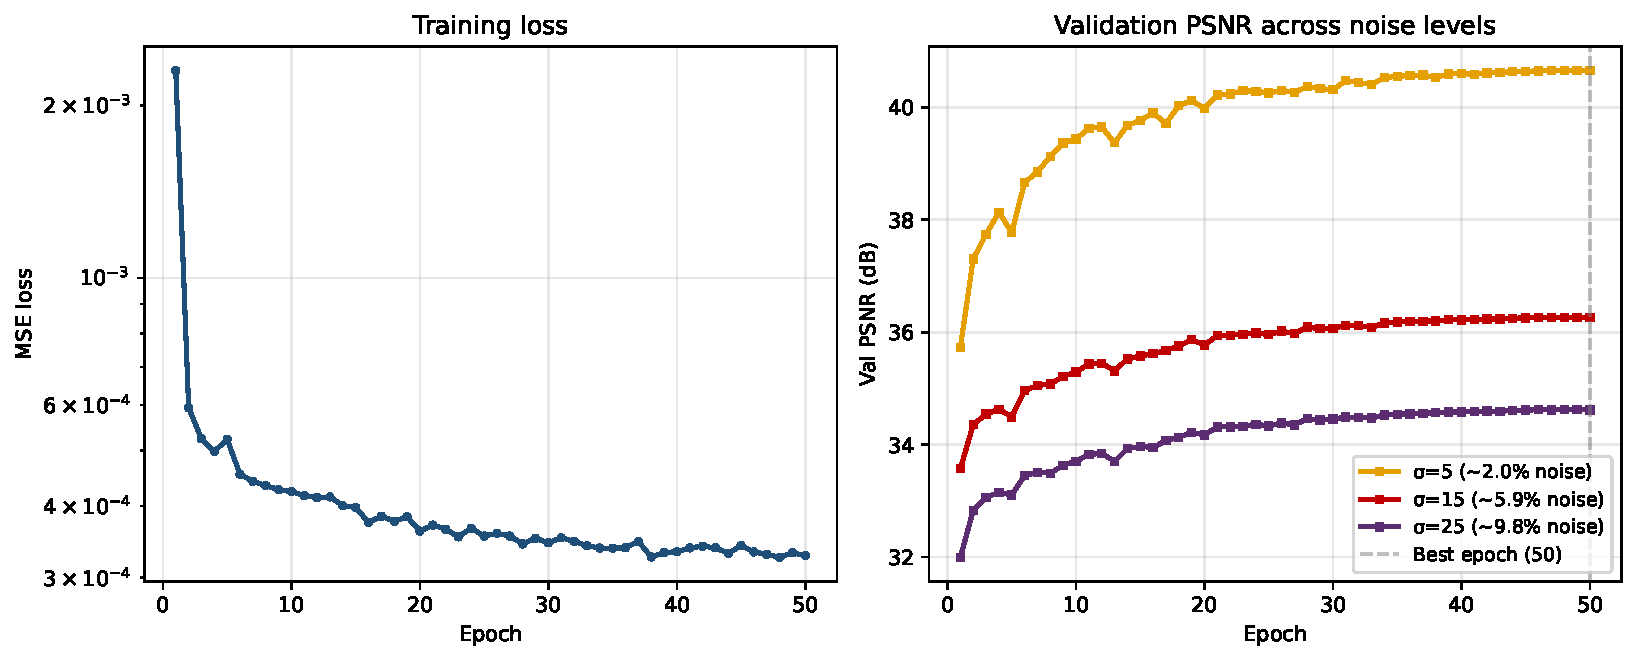
\includegraphics[width=\linewidth]{../figures/12/04_full_training_curves.pdf}
    \caption{CT-DRUNet training curves. Left, MSE loss on the LIDC
    training split over 50 epochs. Right, validation PSNR at
    $\sigma \in \{5, 15, 25\}$. Best checkpoint selected by peak
    validation PSNR at $\sigma = 15$.}
    \label{fig:ct_drunet_training}
\end{figure}

% ============================================================
%  Section 3.7 — Compute infrastructure
% ============================================================
\section{Compute infrastructure}
\label{sec:compute}

All experiments were run on the Cambridge Service for Data Driven Discovery (CSD3) HPC cluster, using GPUs on the \texttt{ampere} partition. GPU access was allocated through a single account, \texttt{MPHIL-DIS-SL2-GPU}, which limited the number of ablation runs and rescue attempts feasible within the project timeline. All jobs were managed through SLURM, with a project-specific conda environment (\texttt{mphil\_ct}) providing the LION toolbox, PyTorch, tomosipo, and supporting packages.

% ============================================================
%  Section 3.8 — Summary of implementation differences from Wei et al.
% ============================================================
\begin{table}[H]
    \centering
    \footnotesize
    \caption{Implementation choices differing from \citet{Wei2022TFPnP}.}
    \label{tab:implementation-differences}
    \begin{tabular}{L{3.5cm}L{3cm}L{3cm}L{4cm}}
        \toprule
        Aspect                & \citet{Wei2022TFPnP} & Ours & Reason \\
        \midrule
        CT geometry            & 30-view TorchRadon        & 30-view custom LION \texttt{Geometry}  & LION had no matching preset \\ \hline
        Detector count         & 182                       & 724 ($\lceil 512\sqrt{2}\,\rceil$) & Cover image diagonal without truncation \\ \hline
        Forward projector      & TorchRadon                & LION + tomosipo & LION native \\ \hline
        Policy backbone stem   & $3\times3$                & $7\times7$ (torchvision default) & Stage widths and $/32$ downsampling unchanged; retraining to match was outside the compute budget \\ \hline
        Value network          & Policy feature extractor with weight norm + TReLU & Eight residual blocks at width 64, no normalisation, standard ReLU & Simpler BN-free critic \\ \hline
        Policy input resolution & $128\times128$           & $512\times512$ native slice & ADMM state passed at full resolution \\ \hline
        Image intensity scale  & [0, 1] normalized         & Native $\mu$ & Preserve physical units \\ \hline
        z-step gradient norm   & None                      & Normalized $A^{\top}r$ & Compensate LION operator scaling \\ \hline
        PSNR data range        & Not stated (likely 1.0)   & Per-image $x_{\text{gt}}.\text{max}()$ & Matches~\texttt{data\_range} in LION conventions \\ \hline
        PSNR / SSIM backend    & Not specified             & Custom PyTorch reimplementations of LION reference & Differentiability for ADMM step \\ \hline
        HaarPSI backend        & Not used                  & \texttt{piq} library & Compatible with $\mu$-unit inputs \\ \hline
        Policy $\sigma$ range  & Not stated                & $[1, 5]$ & Calibration for natural DRUNet \\ \hline
        Policy $\mu$ range     & Not stated                & $[10, 100]$ & Effective range post-gradient-normalization \\ \hline
        Denoiser training data & BSD400 natural images     & Same (\texttt{run\_04}) LIDC (\texttt{run\_11}) & In-domain extension \\ \hline
        Denoiser $\sigma$ range & $[1, 50]$                & $[0, 50]$ (\texttt{run\_11}) & Following~\citet{zhang2021plug} \\ \hline
        Denoiser loss          & $L_1$                     & MSE  & Simpler default, PSNR-aligned \\ \hline
        Denoiser batch size    & 32                        & 8    & Fits GPU budget \\ \hline
        Policy learning rates  & $l_\theta{=}10^{-4}$, $l_\phi{=}5{\times}10^{-5}$ (later halved) & Critic $10^{-4}$, policy $3{\times}10^{-5}$, param $10^{-6}$ & Empirical stability with our action ranges \\ \hline
        Policy training data   & PASCAL VOC natural images & LIDC (all runs) & In-domain policy training \\ \hline
        FBPConvNet training noise & Mixed (implied by flat PSNR) & 5\% fixed & Simplest testable regime \\ \hline
        Test set               & COVID-19 lung, 50 images  & LIDC-IDRI, 389 images & LION-native dataset \\
        \bottomrule
    \end{tabular}
\end{table}

% ============================================================
%  Section 3.9 — Evaluation metrics
% ============================================================
\section{Evaluation metrics}
\label{sec:metrics}
Reconstruction quality is evaluated using peak signal-to-noise ratio (PSNR)~\citep{Wang2004SSIM}, structural similarity index (SSIM)~\citep{Wang2004SSIM}, and Haar wavelet-based perceptual similarity index (HaarPSI)~\citep{Reisenhofer2018HaarPSI}. PSNR is the standard metric used by~\citet{Wei2022TFPnP} and is essential for direct comparison to their reported results. The motivation for reporting SSIM and HaarPSI alongside PSNR is discussed in~\Cref{sec:metrics-discussion}.

PSNR and SSIM are reimplemented in PyTorch to preserve differentiability through the reward computation chain, which is required for the model-based $\pi_2$ policy gradient's backpropagation through the ADMM environment. Both reimplementations follow LION's per-image convention using \texttt{data\_range}$= x_{\text{gt}}.\text{max}()$. HaarPSI is used only at evaluation time, so no custom implementation is required, allowing it to be loaded from the \texttt{piq} library~\citep{Kastryulin2022PIQ}, which accepts a configurable \texttt{data\_range} compatible with our $\mu$-scaled inputs. LION's own HaarPSI implementation requires inputs strictly in $[0, 1]$ and was not used to avoid per-image normalisation. All metrics are computed per-image and averaged over the test set.

% ============================================================
%  Section 3.10 — Reproducibility difficulties
% ============================================================
\section{Reproducibility difficulties}
\label{sec:reproducibility-difficulties}

Several aspects of~\citet{Wei2022TFPnP}'s methodology were ambiguous or underspecified, requiring interpretation during reproduction. The paper does not explicitly state the PSNR data range convention, the baseline TV solver, the FBPconv training regime, or the ADMM $z$-step solver used for CT. The choices made in each case are documented in~\Cref{tab:implementation-differences}.

\textbf{Reference code differences.} The paper's forward operator uses TorchRadon~\citep{Ronchetti2020TorchRadon}, which returns sinograms already scaled by the ray-length correction. LION's tomosipo-based operator does not apply this correction, propagating the mismatch through the pipeline and requiring FBP normalisation, ADMM gradient scaling (the $\mu$ range), and the SCALE factor in noise generation (\Cref{sec:geometry-noise}).

\textbf{RL training stability.} When the $\sigma$ range was widened from $[1, 5]$ to $[1, 15]$ to accommodate the CT-trained DRUNet in \texttt{run\_11}, the critic loss exploded around policy update step 15{,}000 and the policy $\sigma$ output collapsed (\Cref{sec:run11}). Our value network is not the one specified in Table~1 of~\citet{Wei2022TFPnP}, so this instability cannot be attributed to the paper's formulation. Stabilising RL training with widened action ranges under our critic requires careful hyperparameter tuning (\Cref{sec:in-domain-gap}).

\textbf{What worked well.} \citet{Wei2022TFPnP}'s reward function ($r = \Delta\text{PSNR} - \eta$), MDP formulation, and Algorithm~1 were sufficiently clear to reproduce directly, and the two-network policy--value architecture is straightforward to implement. The reproduction follows the paper's algorithm closely and produces results within the paper's reported range, subject to the architectural deviations recorded in~\Cref{tab:implementation-differences}.